\begin{figure}[!htbp]
\centering
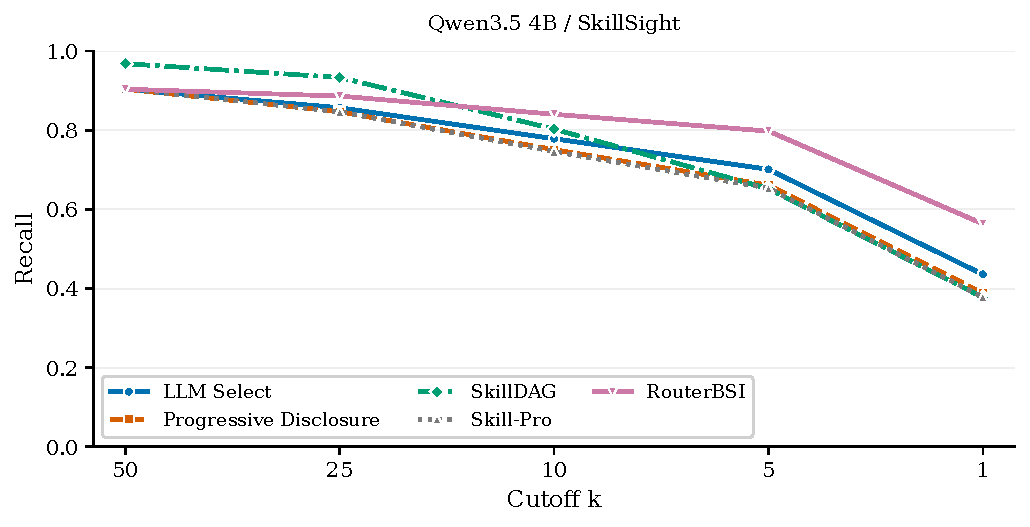
\includegraphics[width=\linewidth]{figs/skillsight_recall_degradation/preview.pdf}
\caption{Average recall under progressively smaller ranked cutoffs, with equal weights across BM25, Vector, and SkillSight. The baseline curve averages the three retrievers' native baselines; every other curve averages the corresponding method across retrievers. Curves show absolute Recall@k, not normalized loss, at equally spaced categorical cutoffs 50, 25, 10, 5, and 1. Each retriever's scores are source task-weighted averages over 748 test tasks; no uncertainty is estimated. Recall retention at cutoff 5 is 100 times Recall@5/Recall@50, computed separately for each retriever and then averaged equally across retrievers. It is not mean per-task retention or a count of retained skills. Skill-Pro ranks selected candidates first, then by retrieval score and original rank; SkillRouter uses its full 50-candidate reranking, not its top-1 selected set. Other archived rankings are retained; differing candidate pools are not a controlled shared-candidate comparison. Vector RouterBSI uses final iteration 10 from the fixed run.}
\label{fig:skillsight_recall_degradation}
\end{figure}
